\chapter{Appendix D: Supplementary Neuromechanical Verification}\label{app:simulation_verification}
\graphicspath{{../Figures/95-AppendixD/}{figs/95-AppendixD/}}

This appendix provides the configuration details and secondary tests supporting Chapter~\ref{ch:sns}. The evidence follows the construction of a neuromechanical experiment: check the mechanical model and signal interfaces, verify individual neural implementations, calibrate and test a selected controller, and examine its responses to controlled interventions. Historical comparisons are identified separately from the revised controller's current results. Neuron equations and spiking calibration remain in Appendix~\ref{app:neuron_equations}.



\section{Mechanical-Model and Interface Verification}\label{sec:app_conversion_repairs}

The conversion workflow involved two distinct problems: importing the robot's artificial-muscle routing with human muscle parameters, and repairing the converted human reference used for controller development. The first combination failed muscle-equilibrium checks because the routed lengths were incompatible with the retained human parameters. The subsequent human-model repairs described below belong to that reference-model loading path; they are not evidence that the BPA-routed model reproduces every human muscle force.

\subsection{Conversion Repairs and Mechanical Checks}

\paragraph{Joint directions and coordinate conventions.}
Single-actuator tests exposed reversed hip-flexion and hip-adduction actions. The corresponding hinge-axis directions were negated so that the muscle actions agreed with the adopted OpenSim conventions. The knee required a different treatment: its converted flexion-negative convention was retained. Rotating the knee without updating its coupled translational coordinates gives a misleading geometry comparison, so those coordinates must follow the prescribed coupling during a pose or actuator test. These are specific joint and path checks, rather than a change from a left-handed to a right-handed model.

\paragraph{Small muscles and force scales.}
The quadratus femoris, gemelli, and piriformis actuators were disabled on both sides. Their six entries remain in the 92-actuator model, with no force contribution. A separate check found eight muscle-actuator entries with an active maximum-force scale of only \qty{1}{\newton}. Their active-force scales were restored from the source-model values. Table~\ref{tab:app_force_scale_repairs} lists the corrected values; each applies separately to the left and right actuator.

\begin{table}[htbp]
\centering
\caption{Active maximum-force scales restored in the converted human model.}
\label{tab:app_force_scale_repairs}
\begin{tabular}{@{}lrr@{}}
\toprule
Muscle & Converted scale (\unit{\newton}) & Restored scale (\unit{\newton}) \\
\midrule
Erector spinae & 1 & 2500 \\
Internal oblique & 1 & 900 \\
External oblique & 1 & 900 \\
Extensor hallucis longus & 1 & 162 \\
\bottomrule
\end{tabular}
\end{table}

These are source-model maximum-force parameters, not measured BPA capacities or the realized force at every pose. The passive-force scales already contained the source values. The converted length ranges for these entries remain a limitation, so restoring the active scale alone does not establish full force--length agreement.

\paragraph{Patella-related paths and coupled joints.}
The converted moving muscle-path points use joints coupled to knee angle. Their sampled limits conflicted with the coupling constraints away from the sampled pose, producing large constraint forces and restricted motion. The coupled path-point joints were therefore left without those conflicting limits while retaining their prescribed trajectories. The anatomical driver joints were treated separately: limits were re-enabled on 14 hinges using the converted ranges. The rectus femoris route also lacked the patella tracking needed for knee-extension action; its intermediate path point was replaced by the vastus medialis patella-tracking point. The force comparison below quantifies the remaining differences at matched poses and activations.

\paragraph{Contact and virtual geometry.}
The converted model contained 19 explicit ground--body contact pairs, independent of geometry contact flags. Suspended tests remove these pairs; ground-contact tests retain only the six foot--ground pairs. Path-marker geometry is noncolliding. These settings isolate intended foot loading from unintended contact with other model components.

These checks verify specific joint actions, coupled paths, and intended contacts. They retain the rigid-tendon approximation and do not establish full OpenSim equivalence or walking; the matched-pose force comparison below quantifies the remaining discrepancies.


\subsection{Matched-Pose Force Comparison}
\label{sec:muscle-models-compare}

The comparison script reads OpenSim static-optimization forces and activations and assigns the corresponding poses and activations to the converted MuJoCo model. It calls the forward calculation at each pose; it does not assign the trajectory velocities or integrate muscle activation and fiber dynamics through time. OpenSim static optimization likewise solves frame-by-frame force allocation rather than a compliant-tendon forward simulation \citep{opensim_static_optimization_docs}. The comparison therefore tests force predictions along sampled poses at matched activation, not dynamic equivalence or tendon-energy storage.

Figure~\ref{fig:force-compare} shows representative force sequences normalized to each curve's peak. Table~\ref{tab:force-r2} retains the saved per-muscle statistics: $R^2=1-\mathrm{SSE}/\mathrm{SST}$, squared Pearson correlation, and the best-aligning lag in analysis frames. The calculation and saved values are in \nolinkurl{Code/MuJoCo_SNS/spinal/_muscle_force_compare.py} and \nolinkurl{muscle_force_compare.csv}.

\begin{table}[htbp]
  \centering
  \caption{MuJoCo vs.\ OpenSim muscle force along the subject01 walk at
  matched activations. Lag in analysis frames ($\approx 17$\,ms each).}
  \label{tab:force-r2}
  \small
  \begin{tabular}{lrrr}
    \toprule
    Muscle & $R^2$ & shape corr$^2$ & lag [frames] \\
    \midrule
    soleus   & 0.742 & 0.800 & 1 \\
    med.\ gastrocnemius & 0.888 & 0.894 & 2 \\
    lat.\ gastrocnemius & 0.884 & 0.887 & 2 \\
    tibialis anterior & 0.945 & 0.945 & 0 \\
    vastus lateralis & 0.941 & 0.945 & 1 \\
    rectus femoris & $-1.15$ & 0.384 & 0 \\
    semimembranosus & 0.565 & 0.621 & 0 \\
    biceps femoris short & $-0.26$ & 0.868 & 0 \\
    psoas & 0.927 & 0.934 & 1 \\
    gluteus maximus (2) & 0.926 & 0.943 & 1 \\
    tensor fasciae latae & 0.933 & 0.935 & 0 \\
    peroneus brevis & 0.977 & 0.989 & 0 \\
    \bottomrule
  \end{tabular}
\end{table}

Eight of the twelve representative muscles have $R^2$ between 0.87 and 0.98 and mean-force ratios within \qty{10}{\percent}. Soleus and semimembranosus have lower agreement, and the negative $R^2$ values for rectus femoris and biceps femoris short head indicate errors larger than predicting the corresponding mean reference force. Shape correlation alone does not remove those errors. The rectus femoris path was altered during conversion, while the biceps femoris short-head result has a substantial force-scale difference. These observations identify muscles requiring closer inspection; they do not isolate routing, force-law, and velocity effects from one another.

The frame-lag calculation describes alignment of these saved sequences. It cannot establish a physical delay caused by tendon compliance because the comparison does not simulate that mechanism. The results support selected pose-wise force checks, with the reported exceptions, rather than a general claim of equivalence for neural-control studies. A dynamic comparison would require matched velocities, activation histories, and explicitly specified tendon dynamics.

\begin{figure}[htbp]
  \centering
  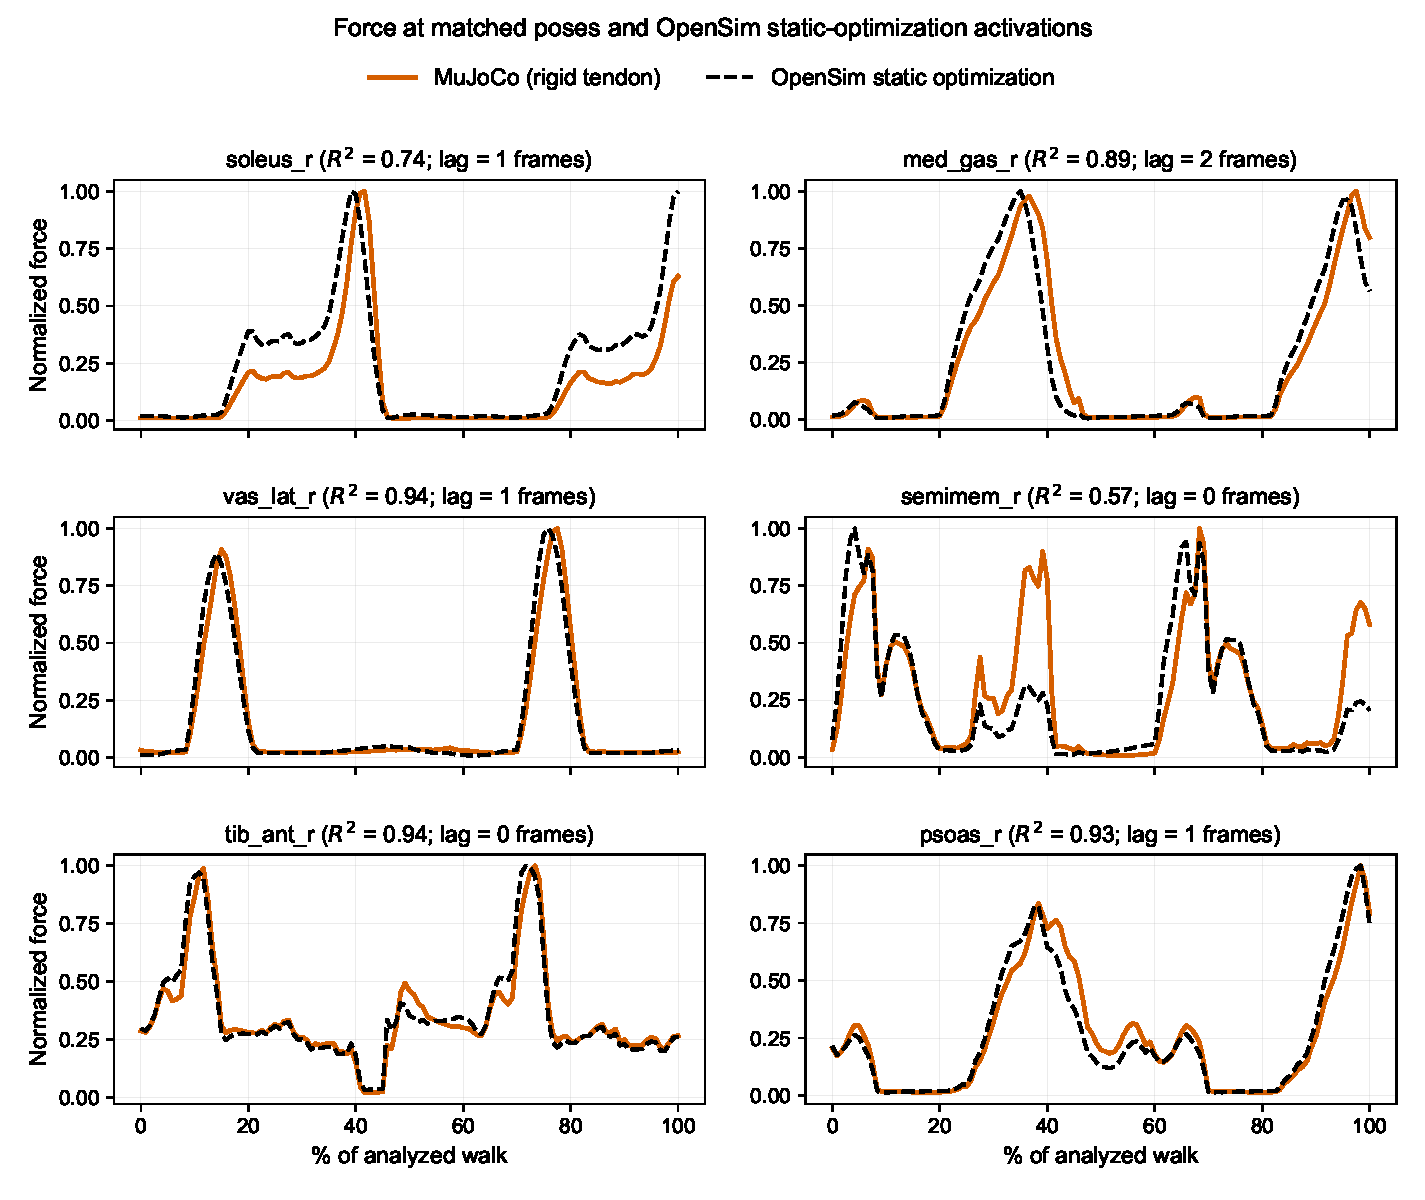
\includegraphics[width=0.9\textwidth]{muscle_force_compare_current.pdf}
  \caption{Force sequences at matched poses and activations, normalized to each curve's peak. Absolute-force agreement is reported in Table~\ref{tab:force-r2}.}
  \label{fig:force-compare}
\end{figure}

\subsection{Neural and Actuator Signal Contracts}\label{sec:app_signal_contracts}

The graphical and programmatic implementations require the same represented quantities, units, signs, and update order at their interfaces. Neural membrane voltages, applied currents, and conductances use millivolts, nanoamperes, and microsiemens, respectively. The neuronal equations and spiking calibration are given in Appendix~\ref{app:neuron_equations}. The one-input SNS-Simscape synapse transmits the pair $[g_k,\,g_kE_k]^{\mathsf T}$ to its postsynaptic neuron, which evaluates
\begin{equation}
I_{\mathrm{syn}}=\sum_k g_kE_k-V\sum_k g_k
=\sum_k g_k(E_k-V).
\label{eq:app_synaptic_contract}
\end{equation}
Here $g_k$ is the conductance calculated from the presynaptic voltage and the specified saturation ramp, and $E_k$ is the reversal potential. Summing these two transmitted quantities within the neuron preserves the conductance-based driving force without a separate postsynaptic-voltage wire to every synapse. The \texttt{SynSum} block combines additional incoming pairs using the same operation.

Motor output, actuator force, and sensory return remain separate interfaces. The biological-muscle block accepts dimensionless activation, musculotendon length in metres, and shortening velocity in metres per second. The characterized BPA blocks accept pressure in kilopascals and path length in metres and return tensile force in newtons. Their mask parameters specify resting, tendon, and fitting lengths. The quasi-static pressure--length force calculation does not supply valve-flow or pressure-transient dynamics. Conversely, the reduced knee demonstration uses its declared simplified actuator law and is not an additional validation of the characterized BPA equations.

The MuJoCo--Simulink bridge exchanges command and measurement arrays between an existing MuJoCo mechanism and a Simulink controller. Each experiment must retain its array ordering, joint sign convention, command scaling, and timestep with its recording. This runtime interface does not translate arbitrary Simscape mechanisms into MuJoCo. The conversion records also identify machine-specific geometry paths and external-source patches that require preflight checking before a fresh MyoConverter run; the demonstrated repaired models are not evidence of a universal one-step conversion process.



\section{Implementation and Circuit-Response Checks}\label{sec:sns_ports}\label{sec:crossengine_methods}

Implementation agreement is assessed with a common circuit specification, identical input samples, and matched update settings. A separate coupled-model test is needed to establish what those neural outputs do to a mechanical model. This distinction also prevents a successful small circuit from conferring verification on a larger controller.

\subsection{Matched Rhythm-Core Implementations}

The contact-driven W2L rhythm-core comparison uses identical neuron parameters, connections, descending drive, and contact inputs in NumPy and Simulink. Burst periods matched at \qty{1.000}{\second}, all ten expected bursts were reproduced, and voltage-trace correlation was at least 0.99996 (Figure~\ref{fig:w2l_crossengine}). Removing the phasic heel inputs caused latching in both implementations. This result verifies the specified input-dependent rhythm core; it does not demonstrate that the circuit oscillates autonomously or that every larger network agrees across implementations.

\begin{figure}[p]
\centering
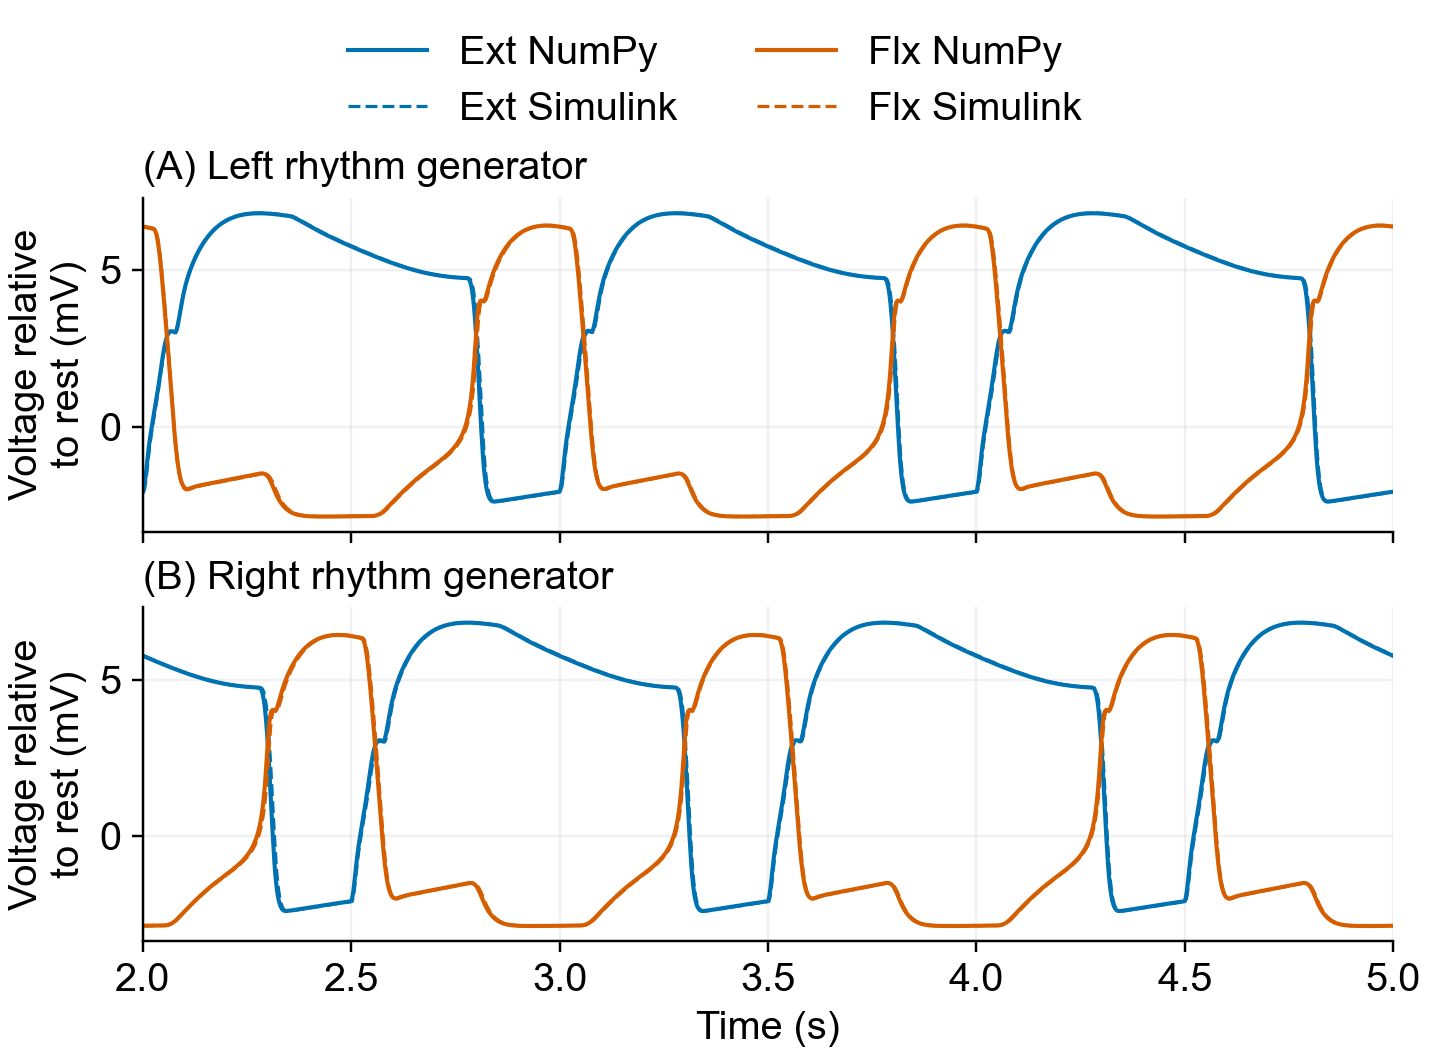
\includegraphics[width=\textwidth,height=0.55\textheight,keepaspectratio]{w2l_crossengine_20261116.png}
\caption[Matched-input W2L rhythm-core comparison]{NumPy and Simulink implementations of the contact-driven W2L rhythm core under identical drive and contact inputs. Agreement concerns the displayed neural circuit and prescribed inputs, rather than independent closed-loop mechanical trajectories.}
\label{fig:w2l_crossengine}
\end{figure}

The separately translated Deng circuit produced a \qty{1.938}{\second} period against a \qty{1.94}{\second} NumPy reference, with antagonist correlation $r=-0.86$. Its archived AnimatLab configuration had an approximately \qty{0.221}{\second} period and an in-phase bilateral rhythm. The parameterizations differ, so antagonist alternation alone does not establish quantitative equivalence. A full 410-neuron export agreed with its NumPy reference to \qty{4.2e-06}{\milli\volt} over the early transient and subsequently diverged. A separate constant-drive realization approached a fixed point while its reference oscillated. These outcomes require configuration-specific verification before parameter transfer.


\subsection{Transient Knee Sensory-Current Response}\label{sec:app_knee_transient}

The knee block model was tested from a settled operating point using a rectangular current pulse added after the spindle transducer and before the extensor Ia sensory-neuron membrane input. Stimulus and no-stimulus cases start from the same initial conditions and run continuously for \qty{50}{\second}; the \qty{2}{\nano\ampere} pulse acts from \qty{30.000}{\second} to \qty{30.030}{\second}. The original configuration did not settle: its knee angle spanned \ang{0.712} during the \qtyrange{25}{30}{\second} baseline window. Its former startup comparison is therefore not used to demonstrate transient reflex recovery.

The graded-response comparison changes exactly six parameters: the two MN output ramp widths from 1 to \qty{10}{\milli\volt}, and the four Ia synaptic ramp widths from 0.5 to \qty{10}{\milli\volt}. Equations, thresholds, conductances, wiring, mechanics, tonic drives, and activation dynamics are retained. This reduces loop gain as an explicit engineering comparison, rather than fitting physiological parameters. The simple actuator-force law is distinct from the characterized BPA model of Chapter~\ref{ch:muscles}. The flexor activation is zero at baseline, so the experiment does not establish suppression of a tonically active antagonist.

The modified configuration passes baseline settling tests for angle, velocity, all six membrane states, and both activations. Its flexion-negative knee baseline is \ang{-42.6392}; positive excursions indicate extension. Extension peaks at \ang{1.0908} after \qty{111}{\milli\second}. Recovery requires displacement within \ang{0.01} of baseline and absolute angular velocity below \qty{1e-4}{\radian\per\second}; both remain within those bounds from \qty{6.355}{\second} after stimulus onset. The late residual is approximately \ang{9.3e-7}. A fresh-process replay reproduces the resampled pulse arrays exactly. Halving the ODE45 maximum step from 1 to \qty{0.5}{\milli\second}, at unchanged tolerances, changes the angle trace by at most \ang{5.21e-5}. Comparisons use linear interpolation onto a \qty{1}{\milli\second} grid, without smoothing. These checks establish numerical recovery in the model, not physiological reflex fidelity. Figure~\ref{fig:app_knee_transient} shows the stimulus, matched kinematics, neural signals, activations, and forces.

\begin{figure}[p]
\centering
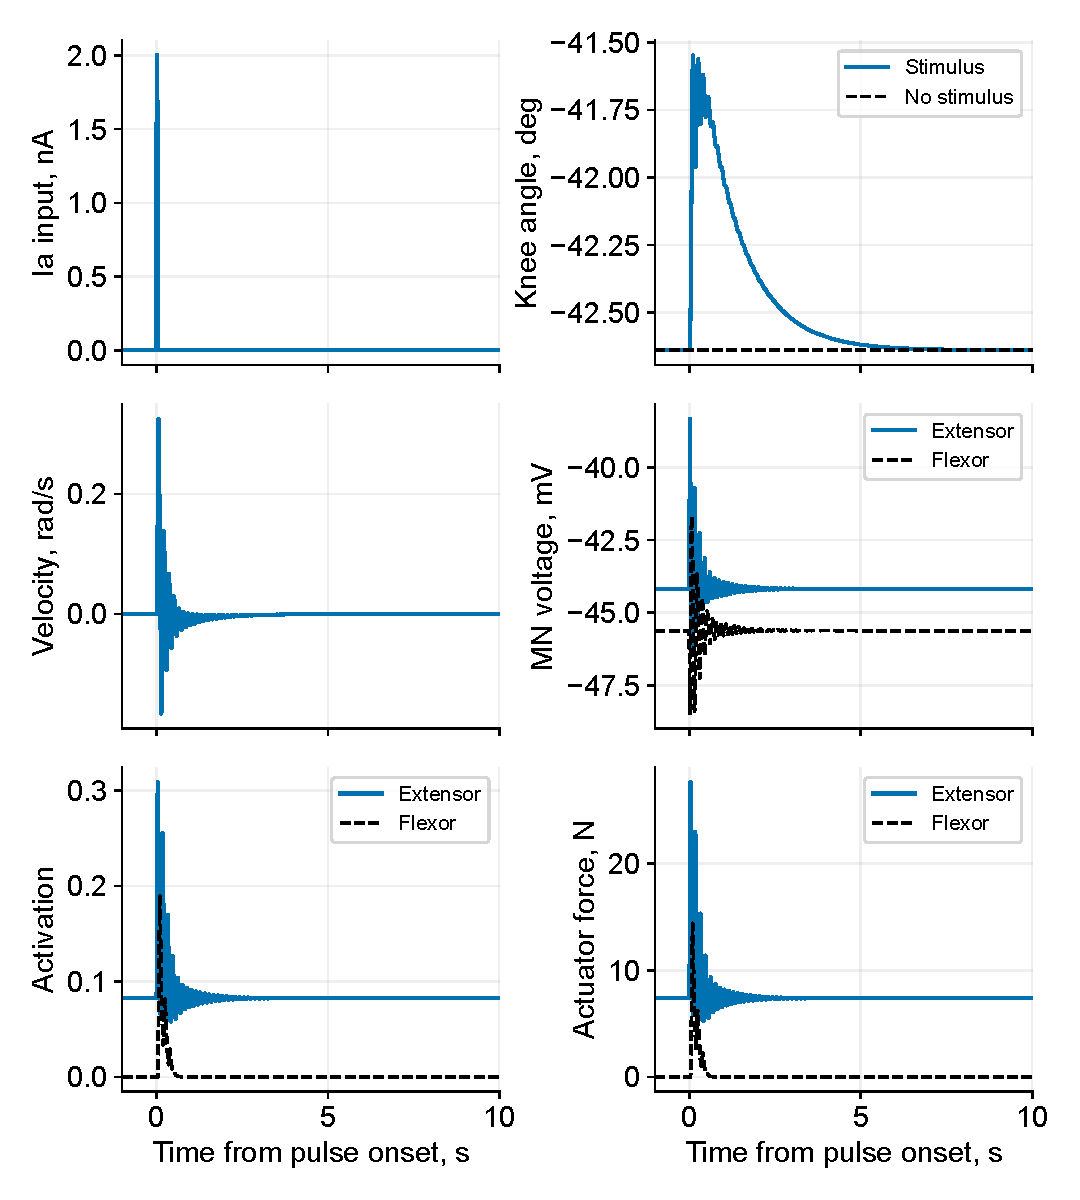
\includegraphics[width=\textwidth,height=0.76\textheight,keepaspectratio]{knee_transient_response.pdf}
\caption[Transient knee sensory-current test]{Stimulus, knee angle, angular velocity, MN voltages, activations, and actuator forces in the graded-response knee model. The pulse enters the extensor Ia sensory neuron after settling. Knee angle is compared with the no-stimulus control; extensor and flexor signals are distinguished in the other paired panels. The display applies only the sign conversion to flexion-negative coordinates.}
\label{fig:app_knee_transient}
\end{figure}



\subsection{A Published Neural Mechanism as a Verification Target}\label{sec:rybak_verification}

The reduced Python implementation of the two-level circuit of \citet{rybak_modelling_2006} passed 13 checks covering drive-dependent activity, repeatability, and the distinction between resetting and non-resetting deletions. Stimulating the pattern-formation extensor population suppressed flexor motor output while the rhythm generator continued, so flexor activity resumed at its expected phase. Stimulating the rhythm-generator extensor population also suppressed flexor output but shifted the subsequent rhythm phase. This comparison tests the functional separation between rhythm generation and pattern formation: similar missing motor bursts can arise through different neural mechanisms. It is a neural-only verification of the translated circuit, independent of a mechanical model and separate from the Simulink demonstrations.



\subsection{Layer-Specific Controls in the Reduced Deng Circuit}\label{sec:app_layer_stimulus}

The fourteen-neuron Deng-derived implementation follows the circuit used in SNS-Toolbox demonstrations \citep{deng_neuromechanical_2019,nourse_sns_2023}. A \qty{0.1}{\milli\second} Euler step reproduced the existing neural integrator's complete \qty{24}{\second} baseline voltage trace exactly in the tested process. The baseline period was \qty{1.938}{\second}. Neural output drove the existing suspended, unilateral W2L mechanical model without afferent return. Hip commands came from the MN outputs; knee and ankle commands used the existing PF-to-activation mapping. This configuration tests transmitted circuit effects, not the original rat mechanics or bilateral walking.

The initial sweep applied \qty{+2}{\nano\ampere} and \qty{+10}{\nano\ampere} to each layer for \qtylist{0.1;0.5}{\second}, together with two direct MN inhibitory controls. None met the deletion criterion. Subsequent stronger-current control series, including stimuli lasting two baseline periods (\qty{3.876}{\second}), retained the same circuit and mechanical parameters (Table~\ref{tab:layer_stimulus}). RG and PF stimuli began one-quarter cycle after a baseline RG onset; MN inhibition began \qty{0.05}{\second} into a baseline motor burst. Positive currents target the extensor RG or hip-PF population; negative currents target the hip-flexor MN. These currents are mechanistic controls, not experimentally calibrated physiological stimuli.

A deletion required at least \qty{20}{\milli\second} of baseline motor activity in the stimulus window and suppression of at least half of that activity, using an activation threshold of 0.5. Phase residuals compare the final four recovered onsets with the nearest baseline onset, normalized by the baseline period. Residuals at or below 0.05 cycles were classified as non-resetting, and those at or above 0.15 as shifted; intermediate values remained indeterminate. RG and motor residuals were assessed separately. The two-cycle stimuli suppressed both expected flexor burst onsets at all three layers. Baseline and stimulated neural and mechanical trajectories were identical before stimulus onset. The \qty{1}{\second} PF pulse shifted the motor pattern without resetting the RG clock, whereas the two-cycle PF pulse preserved both schedules. The duration dependence cautions against treating every motor phase shift as an RG reset. The coupled mechanical traces contained large joint-limit violations, so these tests are interpreted through their neural responses in Table~\ref{tab:layer_stimulus}.

\begin{table}[htbp]
\centering\small
\caption[Layer-specific stimulation controls]{Selected stronger-current controls in the reduced Deng-derived circuit. Phase residuals are fractions of the baseline cycle. ``No deletion'' means the specified suppression criterion was not met.}
\label{tab:layer_stimulus}
\begin{tabularx}{\textwidth}{@{}lrrcc>{\raggedright\arraybackslash}X@{}}
\toprule
Target & \unit{\nano\ampere} & \unit{\second} & RG phase & MN phase & Outcome \\
\midrule
PF & $+50$ & 1.0 & 0.000 & 0.208 & Motor pattern shifted; RG preserved \\
RG & $+50$ & 3.876 & 0.211 & 0.211 & Resetting deletion \\
PF & $+50$ & 3.876 & 0.000 & 0.000 & Non-resetting deletion \\
MN & $-500$ & 3.876 & 0.000 & 0.000 & Non-resetting deletion \\
\bottomrule
\end{tabularx}
\end{table}



\subsection{Archived AnimatLab Models}\label{sec:animatlab_validation}

Headless reruns tested whether archived models reproduced their reference behavior in the original simulator. Eleven targetable rhythm and gait metrics passed their acceptance bands. The bilateral contact-driven model's rhythm generators had periods of \qtylist{0.450;0.467}{\second}; the modern W2L model showed joint oscillations at \qty{2.25}{\Hz}. The Li-model rerun reached \qty{0.637}{\meter\per\second} with step periods near \qty{1.3}{\second} \citep{li_bipedal_2017}. These are reference-model checks, not results for the combined Deng--Li model or evidence of unsupported walking.

A separate MuJoCo translation of the Li controller and body did not reproduce that original-simulator walking result. In a \qty{20}{\second} ground test, mean forward speed was \qty{0.040}{\meter\per\second}, with eleven detected right-foot stance episodes and none on the left. The right-side period of \qty{1.294}{\second} alone therefore did not establish bilateral stepping. This failure distinguishes reproduction of the source model from successful transfer to another simulator.


The original course-project circuit used a shared RG to supply bilateral PF and motor pathways (Figure~\ref{fig:animatlab_shared_rg}). It is retained as the source-model architecture for the motivating transfer attempt, distinct from the later bilateral W2L108 circuit.

\begin{sidewaysfigure}[p]
\centering
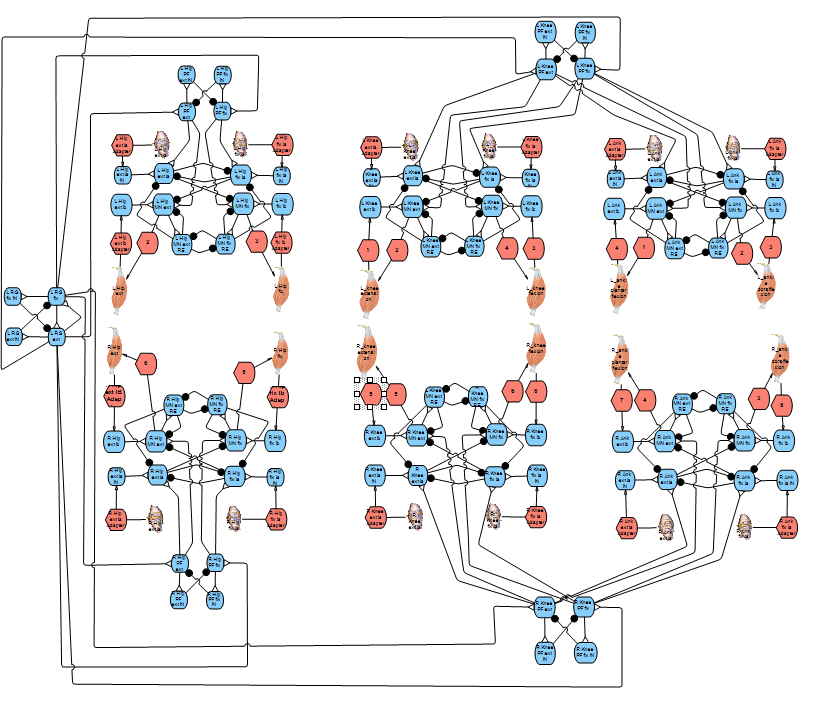
\includegraphics[width=\textheight,height=0.78\textwidth,keepaspectratio]{animatlab_shared_rg_original_20261116.png}
\caption[Original shared-RG controller architecture]{Original course-project shared-RG controller. A common rhythm-generating circuit supplies bilateral hip and knee/ankle pattern-formation pathways and motor outputs. This archived drawing identifies the motivating circuit; the later bilateral W2L controller has a separate RG on each side and additional sensory projections.}
\label{fig:animatlab_shared_rg}
\end{sidewaysfigure}

The earlier instrumented AnimatLab trial records joint, neural, sensory, and body-motion channels over \qty{10}{\second} at a \qty{0.2}{\milli\second} interval. Figure~\ref{fig:animatlab_short_response} retains an aligned short window. Contact-sensory channels are membrane voltages, not contact forces. The initial external horizontal force and absence of a recorded timed vertical release prevent interpreting the run as an independent drop, touchdown, or stable-walking test. The reorganized bilateral project is a different configuration; its completion of simulation runs without sustained alternation is an assembly result.

\begin{figure}[p]
\centering
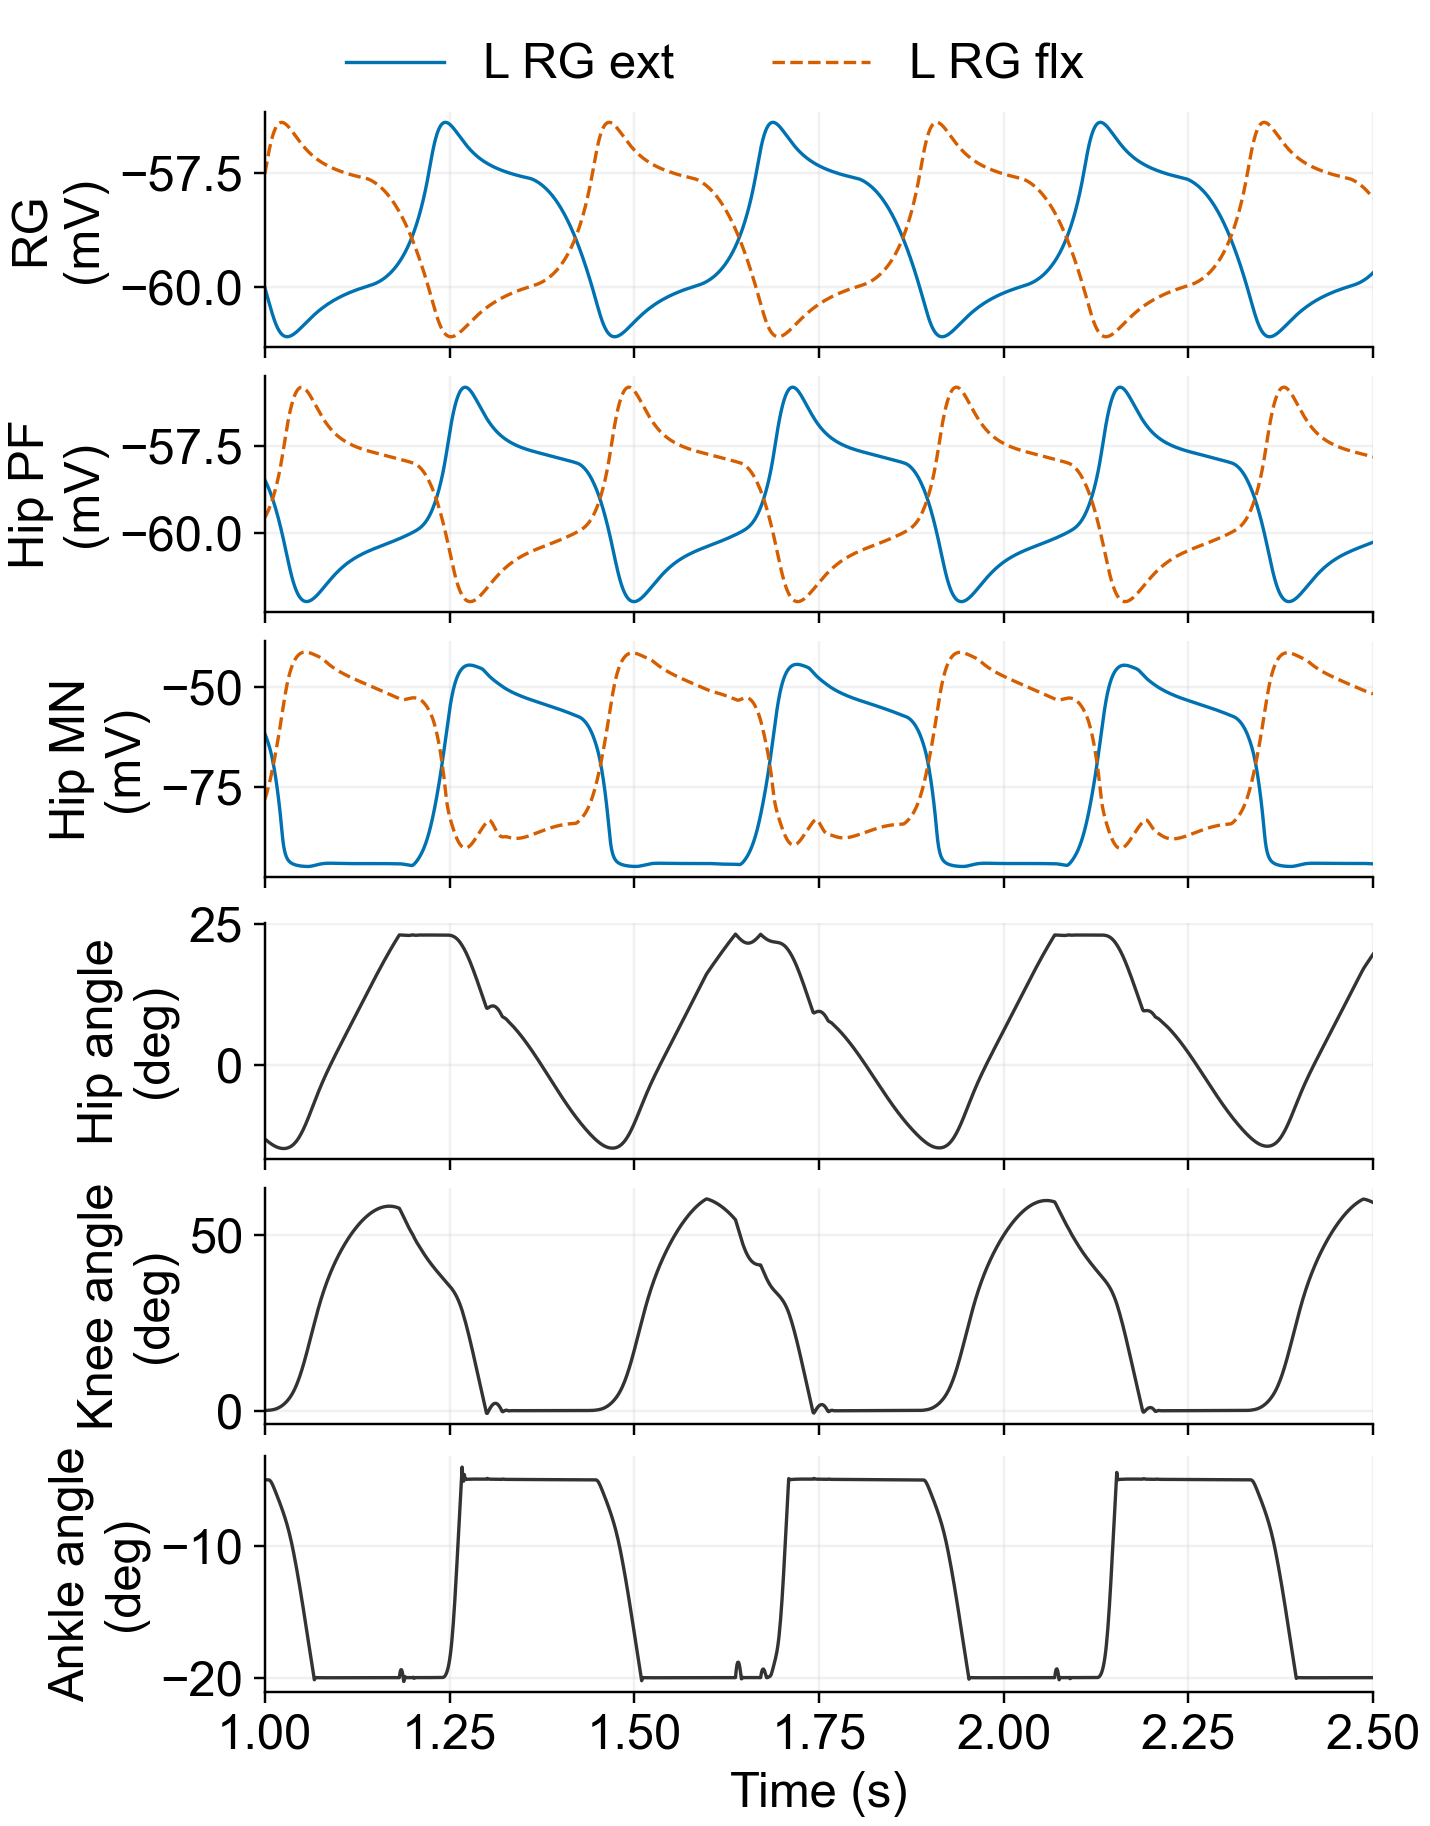
\includegraphics[width=\textwidth,height=0.72\textheight,keepaspectratio]{animatlab_short_response_20261116.png}
\caption[Archived AnimatLab neural and mechanical recording]{Aligned RG, PF, and MN activity and hip, knee, and ankle motion from the same suspended AnimatLab trial over \qtyrange{1}{2.5}{\second}. Extensor and flexor pathways are blue solid and orange dashed. Voltages are graded membrane signals, and the original joint conventions, including positive knee flexion, are retained. This is the earlier instrumented configuration.}
\label{fig:animatlab_short_response}
\end{figure}



\section{Staged Calibration and Coupled-Model Experiments}\label{sec:sns_tuning_methods}\label{sec:sns_curriculum}

Neural calibration and the physical curriculum test different requirements. Ordered neural fits evaluate intrinsic rhythm, timing with expected afferents, feedforward motor recruitment, and local-feedback refinement. Their activation targets are inverse-mechanics estimates from the reference motion, not measured electromyograms. A successful output fit is therefore followed by tests in the actual mechanical model. Each selected configuration retains its source hashes, settings, trial records, matched controls, and independent-process repeat. The physical curriculum separates deafferented air motion, afferented air motion, standing, supported stepping, and contact refinement; completing one stage does not establish the later stages.

The acceptance procedure first checks finite states, completion of the specified duration, anatomical knee bounds, and the required movement. Cadence, bilateral phase, loading, clearance, and assistance are then interpreted for that experiment. The historical gait score's reserved no-cycle value is $-25$; it must be rejected before ranking, since its numerical value exceeds many genuine movement scores. Scores from different configurations are not a common measure of locomotor quality.

\subsection{BiW2Lvar+ Air Stages}\label{sec:app_biw2l_air}

The revised graded BiW2Lvar+ controller completed both air stages with the same learned weights and a shared PF-to-MN expression scale of 0.1. The archived selector \texttt{hunt} is a compatibility identifier for this implementation; Hunt's contribution is the calibration method, not authorship of the controller. Table~\ref{tab:app_air_stages} reports the principal-cycle audit. The \qty{16}{\second} runs use the native MuJoCo biological-muscle formulation and the repaired Gait2392 human model.

\begin{table}[htbp]
\centering\small
\caption[Fixed-controller air-stage evaluations]{BiW2Lvar+ air stages using unchanged learned weights. Phase error is distance from bilateral antiphase in cycles. Negative knee angles indicate flexion. These are suspended-motion tests.}
\label{tab:app_air_stages}
\begin{tabularx}{\textwidth}{@{}>{\raggedright\arraybackslash}Xrrrr@{}}
\toprule
Condition & Cycles R/L & Period (s) & Phase error & \shortstack{Maximum knee angle\\R/L (deg)} \\
\midrule
Deafferented air & 4/4 & 2.466 & 0.0337 & $-1.300/-1.326$ \\
Afferented air & 7/7 & 1.300 & 0.0933 & $-1.718/-1.801$ \\
\bottomrule
\end{tabularx}
\end{table}

The original stage-1 counter counted secondary flexion humps as additional cycles. The preserved principal-cycle audit instead uses autocorrelation and separated principal peaks; its checks accept antiphase double-hump signals and reject synchronous, frozen, and fast test signals. The legacy failed assessment remains in the record. Stage 2 passes both counters. Secondary humps remain a waveform-quality limitation, even when the principal-motion criterion passes.

Ground contact is disabled and measured foot forces are zero. From \qty{5}{\second} onward in stage 2, the suspension spring carries \qty{99.860}{\percent} of body weight, with frontal guidance retained. This measures the apparatus force in an air experiment, not a minimum support requirement for ground walking. Higher-expression trials stopped at the predictive knee-extension guard; the completed condition retains the guard and does not clip joint state. This controller has not completed standing or ground stages.

\subsection{Fixed-Weight Neural Noise and Phase-Specific Stimuli}\label{sec:app_current_noise}\label{sec:app_biw2l_stimulus}

With the stage-2 weights fixed, independent ongoing current noise was applied to four RG cells. Three seeds were evaluated at each stationary standard deviation of \qtylist{0.01;0.025}{\nano\ampere}, with a \qty{20}{\milli\second} correlation time. All six noisy trials completed and retained the principal-motion, knee, and frontal-separation criteria. A zero-noise control and repeated noisy seed also passed. The repeated seed reproduced joint states, neural voltages, and applied noise exactly in a fresh process. This tests the selected air condition under continuous neural-current disturbance; it is distinct from perturbing fixed connection parameters or testing ground balance.

Matched baseline and stimulus runs applied \qty{2}{\nano\ampere}, \qty{100}{\milli\second} pulses separately to RG-F, hip-flexor PF, and iliacus MN, together with a \qty{-2}{\nano\ampere} PF control. Pre-pulse neural trajectories agree exactly. At the silent-PF phase, the excitatory pulse changed PF voltage without crossing its outgoing transmission threshold and produced essentially no MN response. At the active phase, it changed PF voltage by up to \qty{1.14}{\milli\volt} and iliacus MN voltage by \qty{0.16}{\milli\volt}. A direct MN pulse changed its voltage by \qty{1.79}{\milli\volt} and subsequently RG-F voltage by \qty{6.04}{\milli\volt} through the closed neural--mechanical loop. These are paired maximum trajectory differences over the response window, not direct synaptic gains.

\begin{sidewaysfigure}[p]
\centering
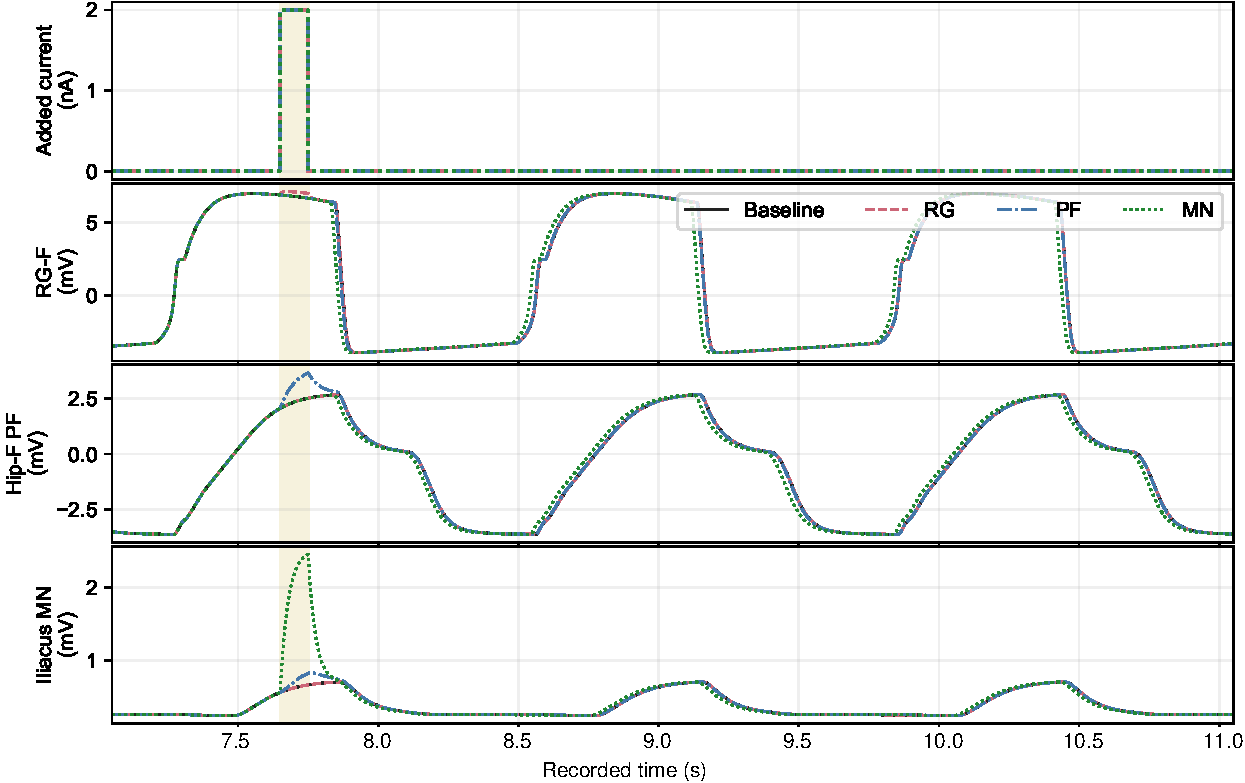
\includegraphics[width=\textheight]{biw2l_stimulus_neural_20261116.pdf}
\caption[Phase-specific interventions in the coupled BiW2Lvar+ model]{Applied current and neural responses to separate RG, PF, and MN pulses in suspended BiW2Lvar+. Each condition retains the same learned parameters and mechanics.}
\label{fig:app_biw2l_stimulus}
\end{sidewaysfigure}

\begin{sidewaysfigure}[p]
\ContinuedFloat
\centering
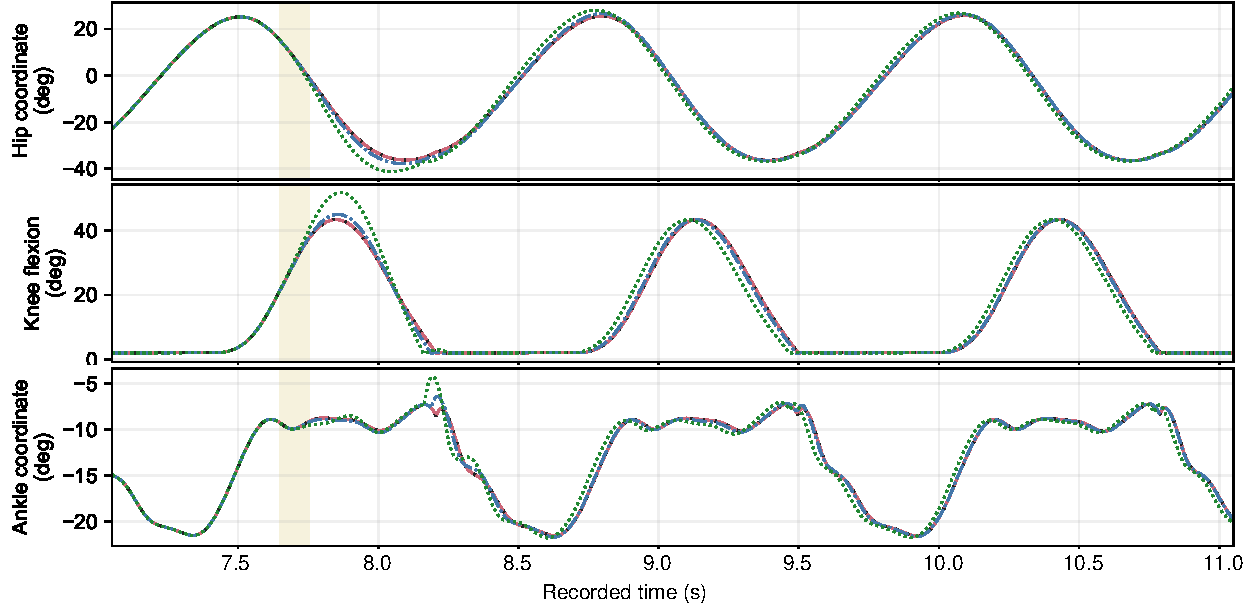
\includegraphics[width=\textheight]{biw2l_stimulus_mechanics_20261116.pdf}
\caption[]{Mechanical responses in the same matched BiW2Lvar+ trials. Time, angles, line identities, and the shaded stimulus interval are unchanged from the source recording.}
\end{sidewaysfigure}

\subsection{A PF-Timing Failure Exposed by Intermediate Verification}\label{sec:app_pf_timing}

Earlier feedforward and feedback output fits for the s3k and syn6 families did not establish that their implemented PF layers produced the intended timing. A subsequent audit evaluated actual outgoing transmission, $\operatorname{clip}(V/\qty{5}{\milli\volt},0,1)$, on the original calibration clock without shifting individual channels to improve alignment. An active threshold of 0.2 defined burst windows. The combined provisional check required absolute fundamental lag no greater than \ang{30}, duty error no greater than 0.15, matching burst counts, and transmission excursion at least 0.2. These are declared engineering acceptance criteria, rather than biological laws.

None of the twelve syn6 channels passed that combined check. Actual centered output variance required three components per side for \qty{99}{\percent} coverage, compared with six for its intended primitive targets. The fifth primitive remained active throughout the cycle on both sides, whereas intended duties were approximately 0.325 and 0.330. The corresponding s3k outputs required two variance components per side, but numerical intended onset and duration windows had not been declared. Variance rank describes the measured waveforms; it is neither a neuron count nor a proof of minimal circuit size. Figure~\ref{fig:app_pf_timing} shows why an acceptable downstream activation fit can conceal inadequate intermediate timing.

\begin{figure}[p]
\centering
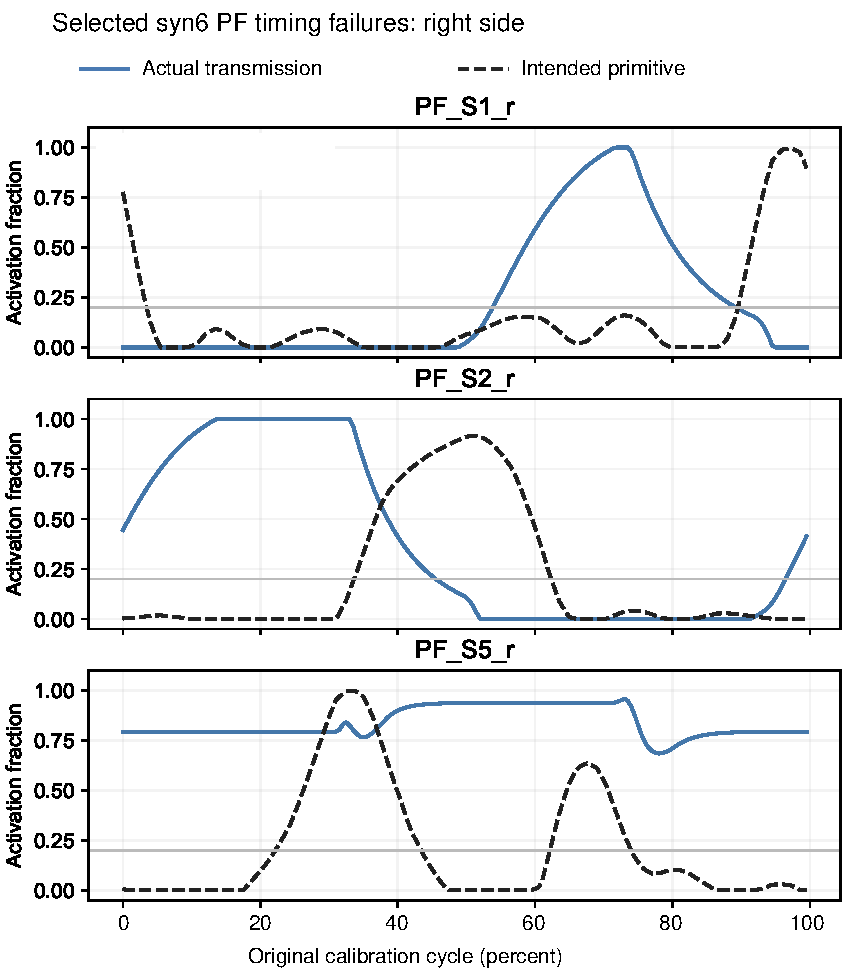
\includegraphics[width=\textwidth]{syn6_pf_timing_selected_20261116.pdf}
\caption[Implemented syn6 PF transmission versus intended primitives]{Representative right-side syn6 PF channels S1, S2, and S5 from the full twelve-channel audit, with unaltered time and transmission coordinates. Solid blue curves show actual transmission; dashed black curves show the intended primitive on the original calibration clock. No individual channel is phase shifted. S1 and S2 show displaced timing, while S5 remains active throughout the cycle. All twelve channels fail the combined provisional check in the full audit. This offline diagnostic is separate from the older-readout syn6 air candidate.}
\label{fig:app_pf_timing}
\end{figure}

A bounded gain-only repair improved the mirrored-target objective and reproduced it in a new process, but still passed zero of twelve channels. It was not accepted or installed in the body adapter. New output-fitting and body-optimization launches for these profiles are held until explicit PF targets, measured timing acceptance, and independent replay have been established. The result identifies a missing intermediate design check; downstream fitting cannot establish that the PF requirement was met.

\subsection{W2L108 Ground Stepping and an Unmet Shuffle Target}\label{sec:app_w2l108_ground}

A separate 108-cell, 216-connection Li--Deng-derived W2L controller was calibrated for its twelve-muscle mechanical body. The selected \qty{10}{\second} trial reproduced all saved numeric arrays exactly in a fresh process and passed its supported ground-stepping criterion with eight left and seven right unloaded, whole-foot-clear swings and alternating qualified transitions. Upward rail/guide assistance averaged \qty{29.519}{\percent} of body weight after \qty{1}{\second}; continuous harness force was zero, but passive rails and slack guides remained. The whole-trial signed assistance of \qty{35.069}{\percent} uses a different window and sign convention and is not a substitute for that upward-force statistic. Its \qty{0.908}{\meter} belt-relative progression is not overground displacement. Peak foot force reached 11.727 body weights, identifying impact transients that still require investigation.

A slower candidate completed \qty{16}{\second}, with seven qualified swings per side and \qty{10.105}{\percent} upward assistance over \qtyrange{2}{16}{\second}. It did not meet the requested short-shuffle criteria: fore-aft excursions were \qtylist{0.351;0.417}{\meter}, and sustained loaded double support occupied \qty{1.929}{\percent} of the analysis window, below the declared \qty{8}{\percent} target. Lower assistance and repeated motion alone therefore did not qualify this candidate. Neither trial is a completion of the five-stage curriculum by BiW2Lvar+.


\subsection{Historical Human-Model Reference Comparison}\label{sec:app_ik_overlay}\label{sec:gait_library_results}\label{sec:walker_variant_results}

The saved human-model controller reproduced its cycle-shape score of $-145.07$ in an independent process. The direct overlay in Figure~\ref{fig:app_gait2392_ik_overlay} uses the Gait2392 walking inverse-kinematics trajectory and its paired ground-reaction-force file. Model cycles begin when vertical foot loading crosses \qty{50}{\newton}; reference stance is defined using the same force threshold. Ten cycles per side, with durations between \qty{0.35}{\second} and \qty{2.5}{\second}, were retained using the existing cycle detector. Each leg was aligned to its own onset and resampled over the gait cycle, without fitting phase, subtracting the mean angle, or scaling amplitude.

Mean cycle periods were \qty{1.285}{\second} on the right and \qty{1.254}{\second} on the left, compared with \qty{1.233}{\second} and \qty{1.213}{\second} in the reference. Model stance fractions were 0.710 and 0.649, compared with 0.610 in the reference. Table~\ref{tab:ik_absolute_rmse} reports absolute-angle errors between mean cycles. These errors retain posture offsets and are distinct from the mean-removed cycle-shape errors used in tuning. The hip and knee show substantial differences in posture and timing, while the ankle trajectories agree more closely. Similar cycle periods therefore do not imply close agreement of the joint trajectories.

\begin{table}[htbp]
\centering
\caption[Absolute-angle errors against Gait2392 inverse kinematics]{Unshifted absolute-angle RMSE between mean model and reference cycles, in degrees.}
\label{tab:ik_absolute_rmse}
\begin{tabular}{lrr}
\toprule
Joint & Right & Left \\
\midrule
Hip & 28.03 & 24.65 \\
Knee & 27.44 & 28.45 \\
Ankle & 8.71 & 7.38 \\
\bottomrule
\end{tabular}
\end{table}

\begin{figure}[p]
\centering
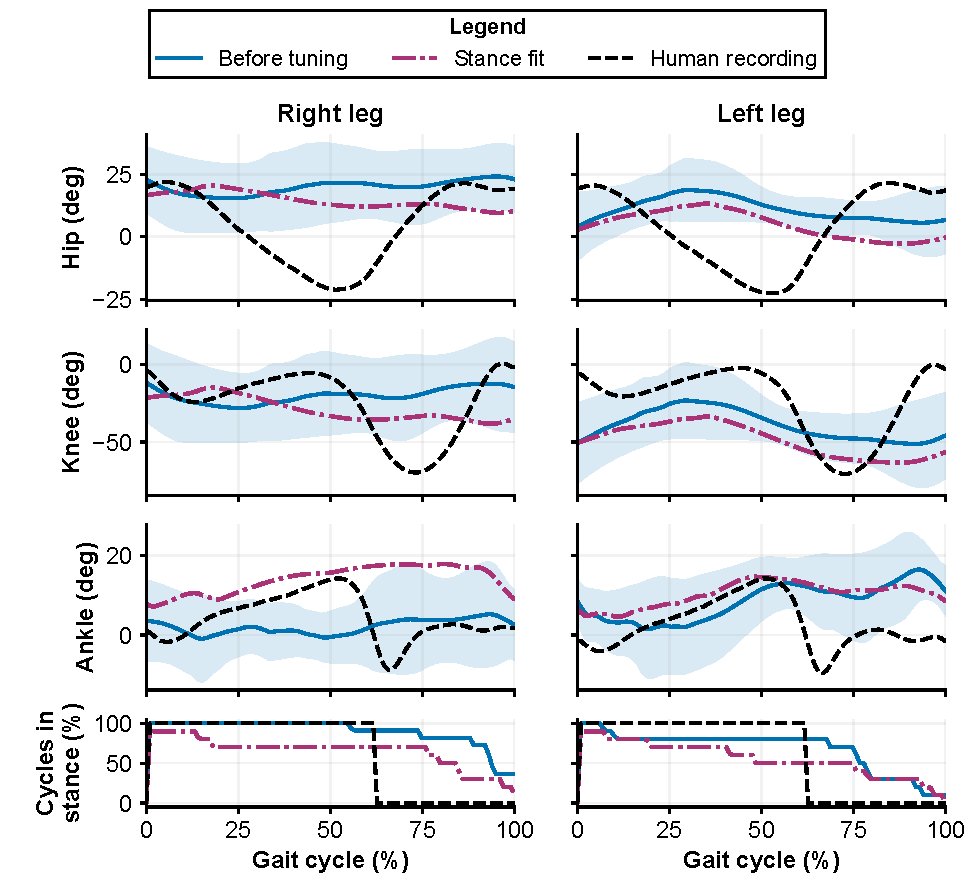
\includegraphics[width=\textwidth]{gait2392_ik_overlay.pdf}
\caption[Direct joint-angle and stance overlay]{Supported Gait2392 human-model motion compared with the inverse-kinematics reference. Columns show the right and left legs. Blue curves and bands show the model mean and one standard deviation across ten cycles per leg; black dashed curves show the reference. Each leg is aligned to its own foot-loading onset, without an angle offset, amplitude adjustment, or fitted phase shift. The bottom row compares model stance fraction across cycles with reference stance and swing, using a \qty{50}{\newton} loading threshold. Absolute-angle errors are reported in Table~\ref{tab:ik_absolute_rmse}.}
\label{fig:app_gait2392_ik_overlay}\label{fig:gait2392_ik_overlay}
\end{figure}


The wider reference set contains 43 cycles, including participant walking and running records and a simulated predicted-walking reference \citep{falisse_modeling_2022}. Comparisons across this set exposed limited transfer and asymmetric activity in the older tuned configurations. Individual pathway removals also had configuration-dependent effects: removing Ia eliminated detected cycles in one production configuration, while all-feedback removal did not have the same effect in every architecture. These older observations motivate matched interventions; they do not certify the later s3k or syn6 PF design or supply ground-stage evidence for the revised BiW2Lvar+ controller.



\section{Supported Evaluations and Controlled Pathway Changes}\label{sec:sns_controller_comparison}

Support conditions, controller identities, and actuator formulations are retained separately when evaluating transfer. In a historical BPA-interface experiment, the nominal support setting was \qty{70}{\percent} of a \qty{411}{\newton} model weight and peak commanded pressure was \qty{372}{\kPa}. This is a quasi-static BPA command/force-interface demonstration. It is distinct from both the native-muscle air trials and the CAD reference-tension results below.

The separate historical robot drive-weaning configuration progressed \qty{1.72}{\meter} in \qty{30}{\second}, retained progression at \qty{60}{\percent} of the supplementary drive scale, and passed twelve perturbed repeats, but did not satisfy the strict contact-duty walking criterion. Its mechanical support was not weaned. In the human-model study, removal of the added left/right hand-drive channels retained bilateral stepping in place under support; the shared locomotor-drive input remained at \qty{2.0773}{\nano\ampere}. Thus zero supplementary drive did not mean zero total descending drive. Neither study established harness-free walking.


\subsection{Independent Replays and Remaining Mechanical Assistance}\label{sec:app_supported_replays}

A separate W2L configuration was evaluated after correcting the delivery of saved per-target gains to the evaluator. Four independent \qty{30}{\second} replays produced identical trajectories. Over the \qtyrange{4.5}{30}{\second} analysis window, the run had 28 left and 21 right contact events, a median bilateral phase of 0.496 cycles, forward displacement of \qty{2.246}{\meter}, and fitted speed of \qty{0.0918}{\meter\per\second}. All twelve independent reruns with \qty{1}{\percent} parameter perturbations passed the supported-stepping criterion. These are results for this configuration, distinct from the drive-weaning configuration.

Removing nominal constant weight support did not remove the position-control harness: its mean vertical force still supplied approximately \qty{16.76}{\percent} of body weight. Contact duty remained below the strict walking criterion. These trials demonstrate repeatable stepping with that remaining assistance. An accelerated neural backend preserved the complete reference trajectories and reduced the isolated neural-step cost by a factor of 1.425; this does not establish the same speed improvement for the complete neuromechanical simulation.

\subsection{Pathway Deletions and Stimulus Tests}\label{sec:app_w2l_perturbations}

The recovered W2L configuration was evaluated with nominal weight support set to 0.25 and the remaining controller settings fixed. Mild and strong drive reductions, forward and backward \qty{40}{\newton} pushes, and separate Ia, Ib, Renshaw, crossed-heel, and heel-cascade deletions retained the supported-stepping criterion. Their effects differed: Renshaw deletion reduced forward displacement to \qty{0.081}{\meter}, while commissural deletion failed bilateral stepping. Disabling all sensory feedback retained joint cycling and \qty{1.996}{\meter} progression but shifted median contact phase to 0.223 cycles, outside the accepted alternation range. The intact comparison produced \qty{2.239}{\meter} and a phase of 0.498 cycles. These experiments distinguish rhythm generation, progression, and bilateral contact coordination, rather than treating them as interchangeable outcomes. Figure~\ref{fig:app_w2l_perturbations} compares the drive, push, and pathway interventions.

\begin{figure}[htbp]
\centering
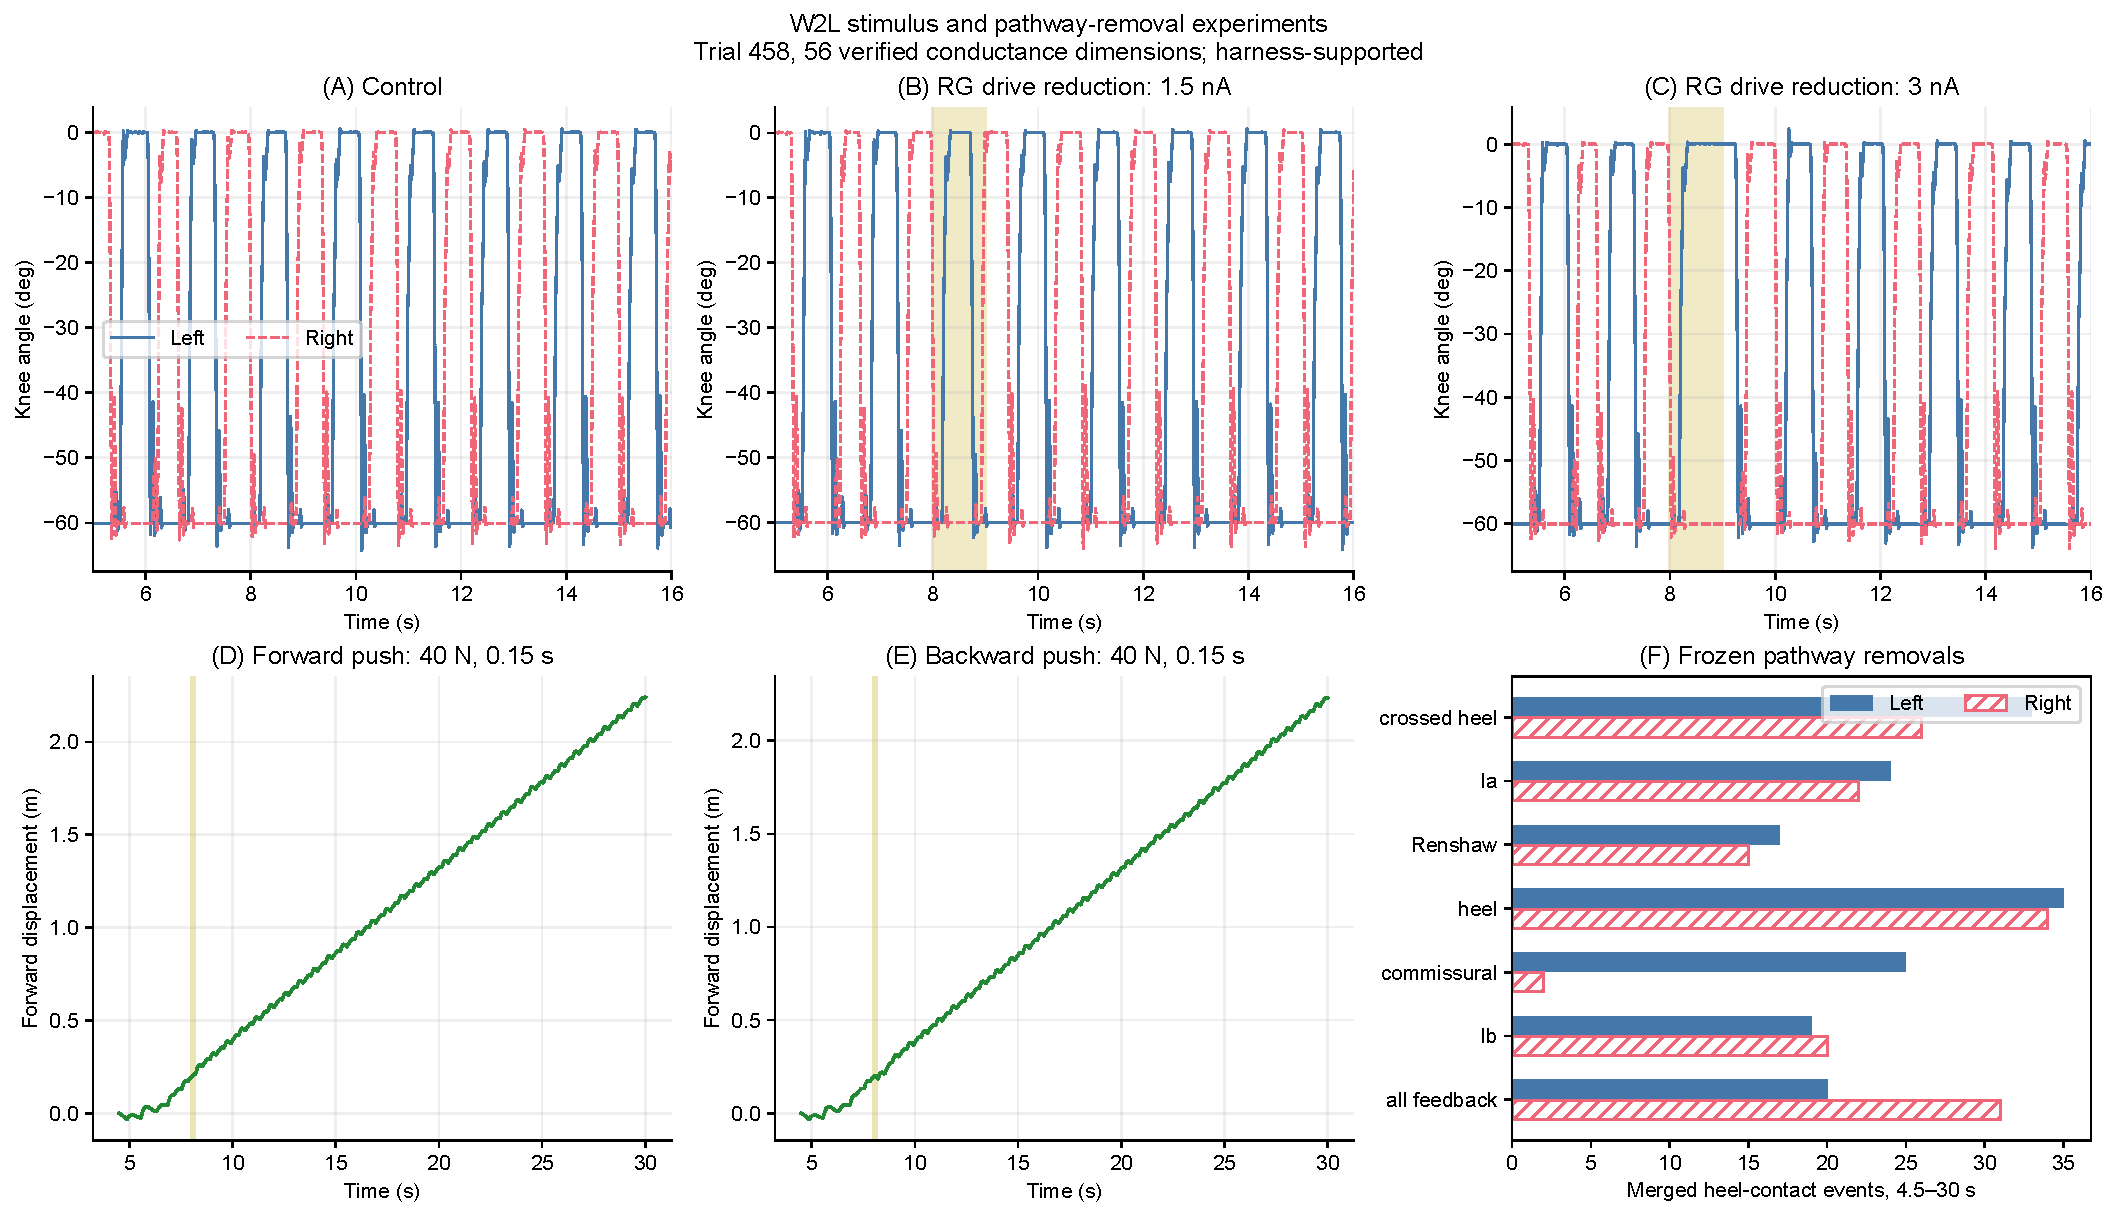
\includegraphics[width=\textwidth]{w2l_perturbation_verified.pdf}
\caption{Recovered W2L controller responses to drive changes, pushes, and pathway deletions. The same effective controller gains are used across conditions, with the specified intervention applied in each panel.}
\label{fig:app_w2l_perturbations}
\end{figure}




\subsection{CAD Robot: Contact Handover and Supported Clearance}\label{sec:app_cad_supported_stance}

The CAD-derived model retains its four-bar knees and spherical hips, using the anatomical frame $x$ anterior, $y$ superior, and $z$ right. The selected controller has 262 graded cells, 230 inputs, and 54 reference-tension actuators. RG activity supplies timing, while an engineering force allocator supplies posture, stance-load, and clearance targets to the MN layer. MN target-current compensation limits normal PF/reflex authority over those outputs. The model therefore evaluates this hybrid architecture, not a complete unmodified neural controller with calibrated dynamic BPA forces.

The latest selected condition completed \qty{28}{\second}. During \qtyrange{16}{28}{\second}, measured vertical harness force supplied \qty{77.5}{\percent} of body weight after the stated support ramp. Seven right and six left qualifying unloaded-clear intervals produced twelve alternations. Each interval required whole-foot mesh clearance above \qty{5}{\milli\meter}, ipsilateral normal load below \qty{7.36}{\newton}, contralateral load above \qty{15}{\newton}, and duration of at least \qty{80}{\milli\second}. Minimum knee flexion was \ang{5.10}, checked at every physics step. The \qty{-74.7}{\milli\meter} world-forward displacement describes guided stepping approximately in place. Orientation and lateral guidance remained active.

Contact handover uses a smooth confidence based on measured load rather than assigning full planned support at initial contact. With $u=\operatorname{clip}[(F-F_0)/(F_1-F_0),0,1]$, confidence is $c=u^2(3-2u)$, using nominal thresholds $F_0=\qty{1}{\newton}$ and $F_1=\qty{5}{\newton}$. Phase preferences are normalized before multiplication by confidence. Requested support is filtered with a \qty{10}{\milli\second} time constant and bounded by the current contact confidence. This calculation allocates muscle targets; it does not apply additional external support.

A swing-clearance task uses measured minimum foot-mesh height and RG-event-derived swing progress to request muscle-mediated lift. Its velocity feedback is part of the task controller, rather than a change in physical joint damping. The bounded allocator maps this task through hip/knee torque targets while excluding root and distal-foot coordinates. The selected condition reproduces all saved arrays in both a fresh repeat and a reference-backend replay. Five of eight local perturbation cases passed; the nominal result therefore does not establish broad parameter robustness. Retained soft contacts still produced transient penetrations of \qtylist{16.13;12.91}{\milli\meter}. Lower-support rungs failed the retained knee guard.

These latest tests supersede the earlier stance-only example as evidence of supported CAD stepping. The older matched separation-control comparison remains a distinct causal test: at unchanged \qty{80}{\percent} assistance, the added controller reduced reversed ankle ordering from \qty{67}{\percent} to zero. It is not a matched comparison with the later \qty{77.5}{\percent} configuration. Route sites can act through ideal rigid offsets outside the CAD surfaces; bracket mass, compliance, packaging, and collision-aware wrapping remain separate verification requirements.



\subsection{Incomplete Literature-Controller Transfer}\label{sec:app_dirusso_attempt}

The Di Russo source mechanical model initialized successfully, but its native custom controller runtime was unavailable for a baseline replay. An exploratory adaptation reproduced its corrected Python equations in a compiled implementation within $3.34\times10^{-16}$ over 2000 steps. Nevertheless, its 960-trial duration-and-speed search selected a tumbling trajectory, which was rejected as walking. Equation agreement did not establish transfer of the source controller's locomotion. The retained source inventory and rejected-run records identify requirements for a future replication; the unsuccessful search is not evidence of walking.


\section{Spiking-Neuron Comparisons}\label{sec:spiking_methods}\label{sec:spiking_results}\label{sec:disc_spiking}

The spiking variants replace afferent, rhythm-generator, and interneuron populations while retaining graded motor neurons. Synapses onto motor neurons are calibrated by mean conductance, preserving the continuous activation interface. This construction does not require the network dynamics or resulting movement to remain unchanged. Calibration and full conversion tables are in Appendix~\ref{app:neuron_equations}.

Action potentials introduce voltage fluctuations absent from a graded signal, so raw membrane-voltage variability is not an equivalent measure of controller output. Figure~\ref{fig:spike_ground} compares filtered neural readouts, muscle activation, and joint motion under the same drive, support, and selected parameters. For a hardware comparison using pulse-width modulation (PWM), both signals would need to pass through the same command encoder and valve limits.

\subsection{MuJoCo Network and Ground Evaluation}

Under constant drive, the non-spiking and spiking rhythm periods were \qtylist{0.399;0.621}{\second}, respectively. The spiking period is \qty{55.6}{\percent} longer. Timing agreement therefore requires more than copying the selected parameters. The historical untuned spiking variant produced bilateral cycling in a supported ground evaluation where the non-spiking winner cycled predominantly on one side (Table~\ref{tab:spike_ground}; Figure~\ref{fig:spike_ground}). This individual comparison motivates further controlled testing; it does not establish superiority of spiking control.

\begin{table}[htbp]
\caption{Supported ground evaluation at the same selected parameters (\qty{16}{\second}), with no spiking re-tuning. The knee minimum is the minimum of the right leg's mean detected cycle. Contact fraction is the fraction of samples with foot normal force above \qty{20}{\newton} during the post-startup evaluation window, whether or not cycles were detected. Thus, the non-spiking left leg can remain in contact for a fraction of 0.985 while completing no detected cycles. The recorded kinematic score summarizes the cycle comparison; less-negative scores indicate closer agreement within this matched test.}
\label{tab:spike_ground}
\begin{tabular}{@{}lcc@{}}
\toprule
\textbf{Metric} & \textbf{Non-spiking winner} & \textbf{Spiking mirror (untuned)} \\
\midrule
Kinematic score                & $-161.57$          & $-236.35$ \\
Gait cycles, right / left      & 9 / 0 (left frozen) & 8 / 9 (bilateral) \\
Cycle knee minimum             & \ang{-64.3}         & \ang{-79.8} \\
Contact fraction, right / left     & 0.637 / 0.985       & 0.799 / 0.856 \\
Maximum pelvis tilt            & \ang{22.1}          & \ang{19.2} \\
Non-finite states              & no                  & no \\
Fell                            & no                  & no \\
\bottomrule
\end{tabular}
\end{table}

\begin{figure}[p]
\centering
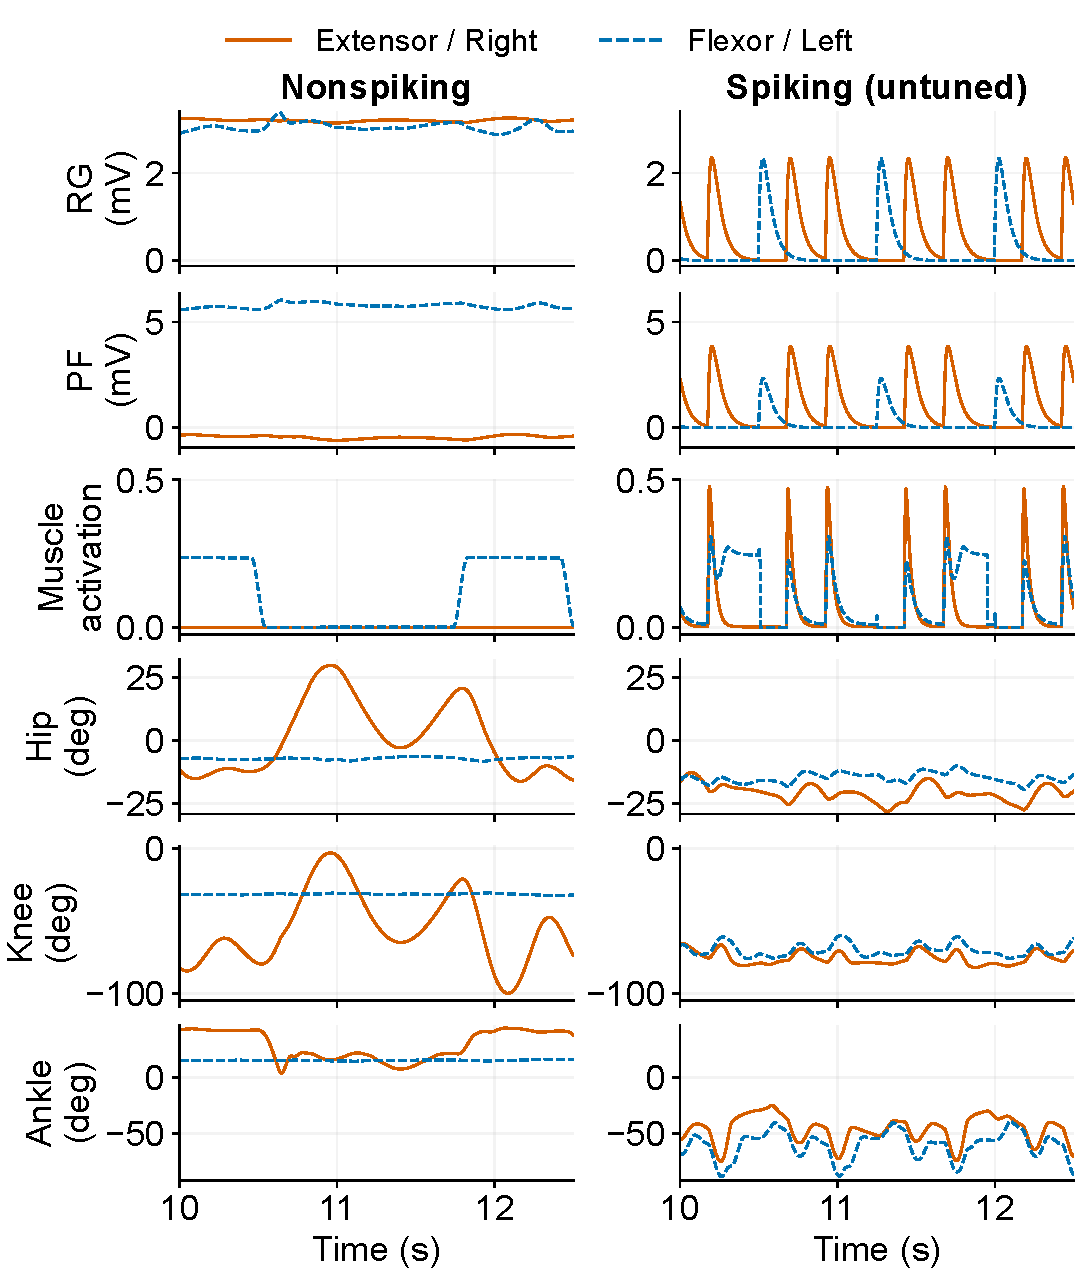
\includegraphics[width=\textwidth,height=0.80\textheight,keepaspectratio]{spiking_ground_neuromechanics_short_20261031.pdf}
\caption[Matched neural and mechanical responses with graded and spiking controllers]{Matched \qtyrange{10}{12.5}{\second} ground-trial window: graded controller (left) and untuned spiking controller (right), at the same selected parameters and support settings. Rows show right-side RG and PF readouts, vastus-lateralis and semimembranosus activation, and bilateral hip, knee, and ankle angles. Neural rows pair extensor (orange solid) and flexor (blue dashed) outputs; joint rows pair right (orange solid) and left (blue dashed) legs. Spiking signals are filtered readouts, and muscle activation is the actuator state.}
\label{fig:spike_rhythm}\label{fig:spike_ground}
\end{figure}

\subsection{Simulink Demonstrations}

The earlier \qty{5}{\second} knee startup comparison used a graded baseline and a spiking twin. Its final-window statistics describe startup activity; the settled, matched-control test in Section~\ref{sec:app_knee_transient} instead measures recovery from a brief sensory-current pulse. The earlier startup figure and its numerical table are retained with the supporting source records rather than repeated here.

In the earlier beverage example, the spiking implementation retained approximately the same sag, \ang{2.02} versus \ang{2.00} in the graded implementation, compared with \ang{7.85} without the reflex. This comparison demonstrates transfer of the tested response after calibration.

\subsection{AnimatLab Conversions}

The tested spiking conversions did not preserve the graded models' rhythm (Table~\ref{tab:spike_animatlab}). Converting thresholds while retaining graded synapses preserved near-baseline oscillations, whereas converting synaptic amplitudes and decay changed or eliminated alternation. These results identify the synapse conversion as a limitation of this mapping. They do not demonstrate that a suitably calibrated spiking implementation cannot reproduce the reference behavior.

\begin{table}[htbp]
\caption{AnimatLab spiking conversions versus their graded baselines (\qty{5.1}{\second} simulations; joint ranges in degrees where the rhythm survives). The thresholds-only ablation converts the neurons but keeps the graded synapses.}
\label{tab:spike_animatlab}
\small
\begin{tabularx}{\textwidth}{@{}p{0.22\textwidth}>{\raggedright\arraybackslash}X>{\raggedright\arraybackslash}X@{}}
\toprule
\textbf{Variant} & \textbf{Baseline (graded)} & \textbf{Spiking copy} \\
\midrule
Two-layer walker     & \qty{0.443}{\second} rhythm;   & no sustained rhythm (2 spikes; \\
                     & hip $-15$ to $+23$, knee $-1$ to $+60$ & hip pinned near $+6$) \\
Bilateral variant    & \qty{0.462}{\second}; antiphase $-0.42$ cycle & sustained unilateral firing; one side at \qtyrange{442}{450}{\hertz} \\
Reorganized project  & no alternation under tonic drives & synchronous \qty{11.8}{\hertz} co-bursting; \\
(standalone export)  &                        & same-leg envelopes $r = 1.000$ at lag 0 \\
Thresholds only      & \multirow{2}{=}{hip $-15$ to $+23$, knee $-1$ to $+60$} & oscillates: hip $-15.1$ to $+23.2$, \\
(graded synapses)    &                        & knee $-0.8$ to $+47.9$ \\
\bottomrule
\end{tabularx}
\end{table}




\section{Execution, Provenance, and Reproduction Tools}\label{sec:app_execution_provenance}

Runtime measurements retain their denominator and experimental scope. One matched complete-process Gait2392 comparison decreased wall time from \qty{199.624}{\second} to \qty{29.284}{\second}, a factor of 6.82, while the neural-update portion decreased from \qty{179.079}{\second} to \qty{9.780}{\second}, a factor of 18.31. Saved trajectories agreed exactly. Neither number should be substituted for a different model, physics configuration, or instrumentation level.

The later compact backend is an incremental comparison against an already accelerated sparse implementation. Warm neural-kernel timing used the median of three 3000-step measurements after an independent 1200-step state comparison in each family. Its largest reported increment was 1.613 for the 1033-cell implementation. In a separate paired \qty{16}{\second} Gait2392 diagnostic run, complete-process times were \qtylist{92.944;91.516}{\second}, giving only a 1.016 ratio. All 62 saved numeric arrays and compiled-model hashes agreed exactly. That single pair includes capture and diagnostics and is not a repeated throughput estimate. The backend retains the existing summation order; unsupported spiking and electrical channels use their existing implementations.

Table~\ref{tab:app_script_map} identifies the executable sources supporting the chapter's tests. Full records preserve configuration, source hashes, compiled model, actual input samples, and aligned neural/mechanical states. A figure can summarize an experiment, but cannot replace those records. Reproduction should use the recorded configuration and environment, then compare arrays before adding a new intervention. Unavailable external raw recordings are identified in the handoff rather than reconstructed from a picture.

\begin{longtable}{@{}>{\raggedright\arraybackslash}p{0.43\textwidth}>{\raggedright\arraybackslash}p{0.52\textwidth}@{}}
\caption[Reproducible implementation and experiment sources]{Relevant source scripts and the tests they support. Prefixes are given below the table. Model builders and test drivers are distinguished from figure-only exporters.}\label{tab:app_script_map}\\
\toprule
\textbf{Source entry point} & \textbf{Role and retained evidence} \\
\midrule
\endfirsthead
\toprule
\textbf{Source entry point} & \textbf{Role and retained evidence} \\
\midrule
\endhead
\bottomrule
\endfoot
\path{convert_to_mujoco.py}; \path{repair_robotbody_muscles.py} (M); \path{runner.py} (P) & Convert source musculoskeletal models, construct the mirrored robot routes, and apply the named human-model loading/repair path. External MyoConverter patches and machine paths require preflight checking. \\
\path{build_ah001.py}; \path{prepare_opensim_routes.py}; \path{build_opensim_routes.py} (C) & Assemble the CAD mechanism and transfer source route points into audited body frames. \\
\path{dynamic_routes.py}; \path{verify_dynamic_routes.py}; \path{verify_knee_tangent.py} (C) & Evaluate moving/conditional sites and verify path derivatives and four-bar tangent kinematics. \\
\path{sns_build_library.m}; \path{sns_build_actuators.m} (S) & Rebuild neural/sensory blocks and pressure--length BPA or biological-muscle blocks; parameterized model sources. \\
\path{sns_units_test_2n.m}; \path{sns_test_actuators.m} (S) & Matched two-neuron calculation and actuator-force checks against the stated equations. \\
\path{demos/sns_build_demo.m}; \path{demos/sns_build_beer_demo.m} (S) & Executable reduced knee and loaded-cup mechanisms and their actual neural pathways. The settled transient protocol is retained separately under \path{results/knee_transient_reflex_20261028/}. \\
\path{sns_build_from_json.m}; \path{sns_verify_from_json.m} (S) & Circuit-specification import and matched-input implementation comparison. \\
\path{mujoco_bridge/matlab/laptop_build_bridge.m} (S) & Build and check the MuJoCo--Simulink runtime bridge; command/measurement exchange, not mechanism conversion. \\
\path{mujoco_bridge/matlab/run_bridge_tests.m}; \path{e1_sns_reflex_loop.m}; \path{e2_cpg_open_loop.m} (S) & Single-muscle, rate, and sensor readback checks, followed by closed-loop reflex and open-loop neural-command demonstrations. \\
\path{_muscle_force_compare.py} (P) & Assign matched OpenSim poses/activations and compute force-comparison statistics. \\
\path{controller_profiles_20261104/campaign.py} (P) & Ordered neural fitting with stored manifests and independent repeats; output fitting is separate from physical acceptance. \\
\path{controller_profiles_20261104/air_validation.py}; \path{dominant_cycles.py} (P) & Actual-body air tests and principal-cycle checks, including rejection controls for the cycle detector. \\
\path{controller_profiles_20261104/noise_trials.py}; \path{stimulus_trials.py} (P) & Frozen-controller current-noise and layer-current interventions; actual input samples retained with aligned states. \\
\path{controller_profiles_20261104/pf_timing_audit.py}; \path{pf_design_gate.py} (P) & Check implemented PF transmission against declared timing targets and prevent downstream promotion after a failed PF-design check. \\
\path{controller_profiles_20261104/diagram_routes.py}; \path{circuit_trace_figures.py} (P) & Draw the compiled circuit and verify routes avoid neuron interiors; drawing checks do not alter circuit equations. \\
\path{w2l_cpg/compact_pairwise_eval.py} (P) & Optional compact neural backend; electrical parity and whole-process timing are checked separately. \\
\end{longtable}

Here M denotes \nolinkurl{Solid_Models/OpenSim/Gait2392_Robotbody/}, C denotes \nolinkurl{Code/MuJoCo_SNS/robot_torso/}, S denotes \nolinkurl{Code/Matlab/SNS_Simscape/}, and P denotes \nolinkurl{Code/MuJoCo_SNS/spinal/}. Where a row gives a directory on the first filename, subsequent bare filenames use that same directory. The portable configuration summaries and source bindings used for the newer experiments are retained under \nolinkurl{Documentation/Reports and Papers/Dissertation/Defense/Session1_Handoff_20261104/}. Raw compiled models and full recordings identified there remain on the originating machine.

\subsection{Hardware Interface Boundary}\label{sec:app_embedded_interfaces}

The \nolinkurl{Code/Hardware/walker_io/} scaffold separates sensor access, afferent encoding, valve commands, communications, and operator supervision. Its modules are \path{sensors.py}, \path{afferents.py}, \path{valves.py}, \path{protocol.py}, \path{lab_console.py}, and \path{orin_daemon.py}. Device readers and the exported SNS update remain unbound. This is a software interface specification for subsequent bench integration, not a measured sensor-to-valve implementation; its proposed timing budget is not hardware performance evidence.
